\chapter{OBJECT DETECTION}

\renewcommand{\headrulewidth}{0.5pt}
\renewcommand{\footrulewidth}{0.5pt}
\thispagestyle{plain}
\pagestyle{fancy}
\fancyhf{}
\fancyhead[L]{\textbf{CHAPTER 2}}
\fancyhead[R]{\textbf{Intelligent Traffic System}}
\raggedright
\fancyfoot[L]{From: ITM Vision}
\fancyfoot[R]{Page \thepage}

\section{Overview}

    \subsection{Traditional Methods}
        \begin{itemize}
            \item Traditional object detection methods are built on handcrafted features and shallow trainable architectures 
            \item Features used in traditional methods: color feature, HOG feature, edge feature, optical flow features, texture features,...
            \item The pipeline of traditional object detection models can be mainly divided into three stages: informative region selection, feature extraction, and classification
        \end{itemize}
    
    \subsection{Deep Learning Based Method}

        \subsubsection{CNNs Overview}
            \begin{itemize}
                \item These methods all take advantage of CNN. CNN uses convolutional layers and pooling layers. Convolutional layers filter inputs for useful information. They have parameters that are learned so that filters are adjusted automatically to extract the most useful information for a certain task. Multiple convolutional layers are used that filter images for more and more abstract information after each layer. Pooling layers are used for limited translation and rotation invariance. Pooling also reduces the memory consumption and thus allows for the usage of more convolutional layers.
                \item Pooling layers provide an approach to down sampling feature maps by summarizing the presence of features in patches of the feature map. Two common pooling methods are average pooling and max pooling that summarize the average presence of a feature and the most activated presence of a feature respectively.
                \item Convolution operation is often interpreted as a filter, where the kernel filters the feature map for information of a certain kind. The convolution operation is usually known as kernels. By different choices of kernels, different operations of the images can be obtained. Operations typically include edge detection, blurring, sharpening etc. A convolutional layer is primarily a layer that performs convolution operation. Its main task is to map. The result of staging convolutional layers in conjunction with the following layers is that the information of the image is classified like in vision.
                \item The pooling layer is responsible for reducing the spacial size of the activation maps. Although it reduces the dimensionality of each feature map, it retains the most important information. There are different strategies of the pooling which are max-pooling, average-pooling and probabilistic pooling.
                \item After several convolutional and max pooling layers, the high-level reasoning in the neural network is done via Fully Connected Layers (FCLs). A FCL takes all neurons in the previous layer and connects it to every single neuron it has. FCLs are not spatially located anymore, that means they can be visualized as one-dimensional.The sum of output probabilities from the Fully Connected Layer is 1. This is ensured by using the Softmax as the activation function in the output layer of the Fully Connected Layer.
                \item A pooling layer is a new layer added after the convolutional layer. Specifically, after a nonlinearity (e.g. ReLU) has been applied to the feature maps output by a convolutional layer; for example the layers in a model may look as follows:
                    \begin{enumerate}
                        \item Input image
                        \item Convolutional layer
                        \item Nonlinearity
                        \item Pooling layer
                    \end{enumerate}
            \end{itemize}

        \subsubsection{Categorize}
            \begin{itemize}
                \item Thanks to Deep Neural Network, a more significant gain is obtained with the introduction of regions with convolutional neural network (CNN) features (R-CNN). DNNs, or the most representative CNNs, act in a quite different way from traditional approaches. They have deeper architectures with the capacity to learn more complex features than the shallow ones. Also, the expressivity and robust training algorithms allow to learn informative object representations without the need to design features manually.
                \item Since the proposal of R-CNN, a great deal of improved models have been suggested, including fast R-CNN that jointly optimizes classification and bounding box regression tasks, faster R-CNN that takes an additional subnetwork to generate region proposals, and you only look once (YOLO) that accomplishes object detection via a fixed-grid regression.
            \end{itemize}

        \subsubsection{Region Proposal Based Method}
            \begin{itemize}
                \item Generate region proposals at first and then classify each proposal into different object categories. Frameworks may be included such as: R-CNN, Faster R-CNN, region-based fully convolutional network R-FCN, feature pyramid networks (FPN), and Mask R-CNN.
                \item Region proposal-based frameworks are composed of several correlated stages, including region proposal generation, feature extraction with CNN, classification, and bounding box regression, which are usually trained separately. Even in the recent end-to-end module Faster R-CNN, an alternative training is still required to obtain shared convolution parameters between RPN and detection network. As a result, the time spent in handling different components becomes the bottleneck in the real-time application.
            \end{itemize}

        \subsubsection{Regression / Classification Based Method}
            \begin{itemize}
                \item Regression/classification based framework solves object detection problem by regarding it as regression or classification problem. Some frameworks may be accounted for examples are: MultiBox, AttentionNet, G-CNN, YOLO, Single Shot MultiBox Detector (SSD), YOLOv2, YOLOv3.
                \item One-step frameworks based on global regression/classification, mapping straightly from image pixels to bounding box coordinates and class probabilities, can reduce time expense.
            \end{itemize}

    \subsection{One Stage Algorithm}

    \subsection{Two Stage Algorithm}

\section{Comparison One Stage and Two Stage}

\section{Comparison YOLO SSD Faster-RCNN}

    \subsection{YOLO}
        \subsubsection{Network Architecture}
            The whole system can be divided into two major components: Feature Extractor and Detector; both are multi-scale. When a new image comes in, it goes through the feature extractor first so that we can obtain feature embeddings at three (or more) different scales. Then, these features are feed into three (or more) branches of the detector to get bounding boxes and class information.
            \begin{figure}[H]
                \centering
                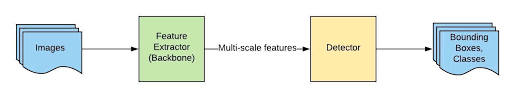
\includegraphics[width=0.8\linewidth]{img/yolo.png}
                \caption{Major components}
            \end{figure}
        \subsubsection{Feature Extraction}
            The feature extractor YOLO V3 uses is called Darknet-53. Darknet-53 contains 53 layers and borrows the ideas of skip connections to help the activations to propagate through deeper layers without gradient diminishing from ResNet. But the Darknet-53 claims to be more efficient than ResNet101 or ResNet152.
            \begin{figure}[H]
                \centering
                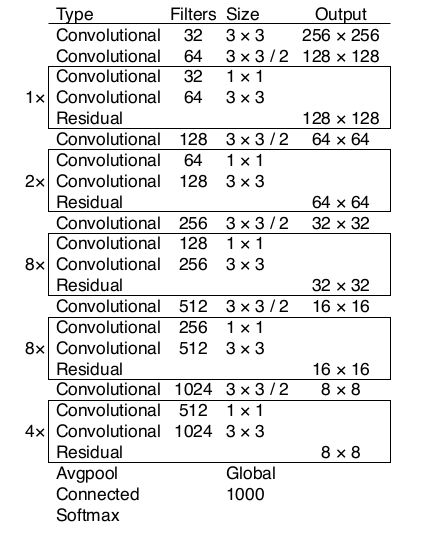
\includegraphics[width=0.8\linewidth]{img/feature_extraction.png}
                \caption{Feature Extraction of YOLOv3}
            \end{figure}
            \vspace{3mm}
            Inside the block, there’s just a bottleneck structure (1x1 followed by 3x3) plus a skip connection. If the goal is to do multi-class classification as ImageNet does, an average pooling and a 1000 ways fully connected layers plus softmax activation will be added. However in the case of object detection, the classification head won't be included, instead, the "detection" head will be added to this feature extractor. Features from last three residual blocks are used in the later detection. 

    \subsection{SSD}

    \subsection{Faster-RCNN}

\section{Metrics and Evaluations}

